\documentclass{beamer}

\usepackage{amsmath}

\usetheme{AnnArbor}
\usecolortheme{crane}
\usefonttheme[onlymath]{serif}

\title{Deep Learning - Foundations and Concepts}
\subtitle{Chapter 4. Single-layer Networks: Regression}
\author{nonlineark@github}
\date{\today}

\begin{document}

\begin{frame}
    \titlepage
\end{frame}

\begin{frame}
    \frametitle{Outline}
    \tableofcontents
\end{frame}

\section{Linear Regression}

\begin{frame}
    \frametitle{Basis functions}
    Consider the linear combinations of fixed nonlinear functions of the input variables:
    \begin{equation*}
        y(x;w)=w_{0}+\sum_{m=1}^{M-1}w_{m}\phi_{m}(x)
    \end{equation*}
    where $\phi_{m}(x)$ are known as basis functions. The parameter $w_{0}$ allows for any fixed offset in the data and is sometimes called a bias parameter. If we define $\phi_{0}(x)=1$ then $y(x;w)$ becomes:
    \begin{equation*}
        y(x;w)=\sum_{m=0}^{M-1}w_{m}\phi_{m}(x)=w^{T}\phi(x)
    \end{equation*}
\end{frame}

\begin{frame}
    \frametitle{Basis function}
    \begin{figure}
        \caption{The linear regression model as a single-layer network}
        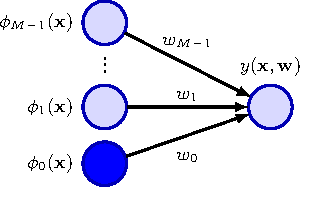
\includegraphics{Figure_1.pdf}
    \end{figure}
\end{frame}

\begin{frame}
    \frametitle{Basis function}
    Here are some possible choices of basis functions:
    \begin{itemize}
        \item Polynomial: $\phi_{m}(x)=x^{m}$.
        \item Gaussian: $\phi_{m}(x)=\exp(-\frac{(x-\mu_{m})^{2}}{2s^{2}})$.
        \item Sigmoidal: $\phi_{m}(x)=\frac{1}{1+\exp(-\frac{x-\mu_{m}}{s})}$.
    \end{itemize}
\end{frame}

\begin{frame}
    \frametitle{Maximum likelihood}
    Consider a data set of inputs $\{x^{1},\hdots,x^{N}\}$ with corresponding target values $t_{1},\hdots,t_{N}$. Assume that given the value of $x^{n}$, the corresponding value of $t_{n}$ has a Gaussian distribution. The likelihood function takes the form:
    \begin{equation*}
        p(t_{1},\hdots,t_{N}|x^{1},\hdots,x^{N};w,\sigma^{2})=\prod_{n=1}^{N}\mathcal{N}(t_{n};w^{T}\phi(x^{n}),\sigma^{2}I)
    \end{equation*}
    The negative log of the likelihood function is given by:
    \begin{align*}
        L&=-\log{}p(t_{1},\hdots,t_{N}|x^{1},\hdots,x^{N};w,\sigma^{2}) \\
        &=\frac{N}{2}\log(2\pi)+\frac{N}{2}\log\sigma^{2}+\frac{1}{2\sigma^{2}}\sum_{n=1}^{N}(t_{n}-w^{T}\phi(x^{n}))^{2}
    \end{align*}
\end{frame}

\begin{frame}
    \frametitle{Maximum likelihood}
    Let's maximize the likelihood function (for simplicity, we will denote $\phi(x^{n})$ by $\phi_{n}$):
    \begin{equation*}
        \frac{\partial{}L}{\partial{}w}=\frac{1}{\sigma^{2}}(w^{T}\sum_{n=1}^{N}\phi_{n}\phi_{n}^{T}-\sum_{n=1}^{N}t_{n}\phi_{n}^{T})=\frac{1}{\sigma^{2}}(w^{T}\Phi^{T}\Phi-t^{T}\Phi)
    \end{equation*}
    where:
    \begin{equation*}
        \Phi=\begin{pmatrix}
            \phi_{1}&\phi_{2}&\hdots&\phi_{N}
        \end{pmatrix}^{T}
    \end{equation*}
    We see that:
    \begin{equation*}
        w_{ML}=(\Phi^{T}\Phi)^{-1}\Phi^{T}t
    \end{equation*}
    The quantity $(\Phi^{T}\Phi)^{-1}\Phi^{T}$ is known as the Moore-Penrose pseudo-inverse of the matrix $\Phi$. It's easy to calculate $\sigma^{2}_{ML}$ as well:
    \begin{equation*}
        \sigma^{2}_{ML}=\frac{1}{N}\sum_{n=1}^{N}(t_{n}-w_{ML}^{T}\phi_{n})^{2}
    \end{equation*}
\end{frame}

\begin{frame}
    \frametitle{Geometry of least squares}
    \begin{figure}
        \caption{Geometrical interpretation of the least squares solution}
        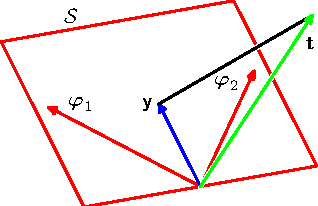
\includegraphics{Figure_3.pdf}
    \end{figure}
\end{frame}

\begin{frame}
    \frametitle{Geometry of least squares}
    Let $\Phi_{m}$ be the $m$th column of the matrix $\Phi$, and let $y_{ML}\in\mathbb{R}^{N}$ be the best approximation to $t$ we obtained by maximizing the likelihood function:
    \begin{equation*}
        y_{ML}=\begin{pmatrix}
            w_{ML}^{T}\phi_{1} \\
            w_{ML}^{T}\phi_{2} \\
            \vdots \\
            w_{ML}^{T}\phi_{N}
        \end{pmatrix}=\Phi{}w_{ML}=\sum_{m=0}^{M-1}(w_{ML})_{m}\Phi_{m}
    \end{equation*}
    Here we clearly see that $y_{ML}\in\mathrm{span}(\Phi_{0},\hdots,\Phi_{M-1})$. In addition, we have:
    \begin{align*}
        &\Phi^{T}y_{ML}=\Phi^{T}\Phi{}w_{ML}=(\Phi^{T}\Phi{})(\Phi^{T}\Phi)^{-1}\Phi^{T}t=\Phi^{T}t \\
        &(t-y_{ML})^{T}\Phi=0\qquad(t-y_{ML})^{T}\Phi_{m}=0
    \end{align*}
    That is, $t-y_{ML}$ is orthogonal to each $\Phi_{m}$, or put another way, $y_{ML}$ is the orthogonal projection of $t$.
\end{frame}

\begin{frame}
    \frametitle{Sequential learning}
    The maximum likelihood estimator for $w$ involves processing the entire training set in one go. Sometimes we want the data points to be considered one at a time and the model parameters updated after each such presentation. The technique of stochastic
    (sequential) gradient descent:
    \begin{itemize}
        \item The error function comprises a sum over data points: $E=\sum_{n}E_{n}$.
        \item After presentation of data point $n$, updates the parameter $w$ using: $w^{(\tau+1)}=w^{(\tau)}-\eta\nabla{}E_{n}$.
        \item $\tau$ denotes the iteration number, and $\eta$ is a training rate parameter.
    \end{itemize}
\end{frame}

\begin{frame}
    \frametitle{Sequential learning}
    For the sum-of-squares error function:
    \begin{align*}
        E_{n}&=\frac{1}{2}(t_{n}-w^{T}\phi_{n})^{2} \\
        \nabla{}E_{n}&=-(t_{n}-w^{T}\phi_{n})\phi_{n} \\
        w^{(\tau+1)}&=w^{(\tau)}+\eta(t_{n}-(w^{(\tau)})^{T}\phi_{n})\phi_{n}
    \end{align*}
\end{frame}

\begin{frame}
    \frametitle{Regularized least squares}
    Adding a regularization term to an error function to control over-fitting:
    \begin{equation*}
        E_{D}(w)+\lambda{}E_{W}(w)
    \end{equation*}
    For example, if we use the sum-of-squares error function, the total error function becomes:
    \begin{equation*}
        \frac{1}{2}\sum_{n=1}^{N}(t_{n}-w^{T}\phi_{n})^{2}+\frac{\lambda}{2}w^{T}w
    \end{equation*}
    Minimizing this total error function, we obtain:
    \begin{equation*}
        w_{ML}=(\lambda{}I+\Phi^{T}\Phi)^{-1}\Phi^{T}t
    \end{equation*}
\end{frame}

\begin{frame}
    \frametitle{Multiple outputs}
    We have considered situations with a single target variable. In some applications, we may wish to predict $K>1$ target variables. Let's first get the dimensions right:
    \begin{itemize}
        \item There are $N$ input data: $x^{1},\hdots,x^{N}$, where $x^{n}\in\mathbb{R}^{D}$.
        \item There are $N$ target data: $t^{1},\hdots,t^{N}$, where $t^{n}\in\mathbb{R}^{K}$.
        \begin{itemize}
            \item Let $T=\begin{pmatrix}
                t^{1}&t^{2}&\hdots&t^{N}
            \end{pmatrix}^{T}\in\mathbb{R}^{N\times{}K}$
        \end{itemize}
        \item There is a basis $\phi$: $\mathbb{R}^{D}\to\mathbb{R}^{M}$, $x\to\phi(x)$. For simplicity, we denote $\phi(x^{n})$ by $\phi_{n}$.
        \begin{itemize}
            \item Let $\Phi=\begin{pmatrix}
                \phi_{1}&\phi_{2}&\hdots&\phi_{N}
            \end{pmatrix}^{T}\in\mathbb{R}^{N\times{}M}$
        \end{itemize}
        \item There is a matrix of parameters: $W\in\mathbb{R}^{M\times{}K}$.
    \end{itemize}
\end{frame}

\begin{frame}
    \frametitle{Multiple outputs}
    Now, let's maximize the likelihood for $y(x;W)=W^{T}\phi(x)$:
    \begin{align*}
        L&=-\log{}p(t^{1},\hdots,t^{N}|x^{1},\hdots,x^{N};W,\sigma^{2}) \\
        &=-\log\prod_{n=1}^{N}\mathcal{N}(t^{n};W^{T}\phi_{n},\sigma^{2}I) \\
        &=\frac{NK}{2}\log(2\pi\sigma^{2})+\frac{1}{2\sigma^{2}}\sum_{n=1}^{N}||t^{n}-W^{T}\phi_{n}||^{2} \\
        \frac{\partial{}L}{\partial{}W}(W)H&=\frac{1}{\sigma^{2}}\sum_{n=1}^{N}(\mathrm{tr}(W^{T}\phi_{n}\phi_{n}^{T}H)-\mathrm{tr}(t^{n}\phi_{n}^{T}H)) \\
        &=\frac{1}{\sigma^{2}}\mathrm{tr}((W^{T}\Phi^{T}\Phi-T^{T}\Phi)H) \\
        W_{ML}&=(\Phi^{T}\Phi)^{-1}\Phi^{T}T
    \end{align*}
\end{frame}

\section{Decision Theory}

\begin{frame}
    \frametitle{Decision theory}
    \begin{itemize}
        \item We have learned from data using maximum likelihood, and the result is a predictive distribution.
        \item However, for many practical applications we need to predict a specific value.
        \item In the inference stage, we use the training data to determine a predictive distribution.
        \item In the decision stage, we use this predictive distribution to determine a specific value.
    \end{itemize}
\end{frame}

\begin{frame}
    \frametitle{Decision theory}
    \begin{block}{Problem}
        Given a predictive distribution $p(t|x)$, determine a specific value $f(x)$, which will be dependent on the input $x$, that is optimal according to some criterion.
    \end{block}
\end{frame}

\begin{frame}
    \frametitle{Decision theory}
    Because we do not know the true value of $t$, we cannot minimize the loss $L=(f(x)-t)^{2}$ itself, instead let's minimize the expected loss:
    \begin{equation*}
        E(L)=\iint(f(x)-t)^{2}p(x,t)\mathrm{d}x\mathrm{d}t
    \end{equation*}
    We want to find $f(x)$ that minimizes $E(L)$:
    \begin{align*}
        \frac{\delta{}E(L)}{\delta{}f(x)}&=2\int(f(x)-t)p(x,t)\mathrm{d}t=0 \\
        f(x)&=\frac{\int{}tp(x,t)\mathrm{d}t}{\int{}p(x,t)\mathrm{d}t}=\frac{\int{}tp(x,t)\mathrm{d}t}{p(x)}=\int{}tp(t|x)\mathrm{d}t=E(t|x)
    \end{align*}
    which is the conditional average of $t$ conditioned on $x$ and is known as the regression function.
\end{frame}

\begin{frame}
    \frametitle{Decision theory}
    Now that we know that the optimal solution is the conditional expectation, we can expand the square term as follows:
    \begin{align*}
        &(f(x)-t)^{2}=((f(x)-E(t|x))+(E(t|x)-t))^{2} \\
        &=(f(x)-E(t|x))^{2}+2(f(x)-E(t|x))(E(t|x)-t)+(E(t|x)-t)^{2}
    \end{align*}
\end{frame}

\begin{frame}
    \frametitle{Decision theory}
    Let's examine the expectation for each term:
    \begin{align*}
        &\iint(f(x)-E(t|x))^{2}p(x,t)\mathrm{d}x\mathrm{d}t=\int(f(x)-E(t|x))^{2}(\int{}p(x,t)\mathrm{d}t)\mathrm{d}x \\
        &=\int(f(x)-E(t|x))^{2}p(x)\mathrm{d}x \\
        &\iint(f(x)-E(t|x))(E(t|x)-t)p(x,t)\mathrm{d}x\mathrm{d}t \\
        &=\int(f(x)-E(t|x))p(x)(\int(E(t|x)-t)p(t|x)\mathrm{d}t)\mathrm{d}x=0 \\
        &\iint(E(t|x)-t)^{2}p(x,t)\mathrm{d}x\mathrm{d}t=\int{}p(x)(\int(t-E(t|x))^{2}p(t|x)\mathrm{d}t)\mathrm{d}x \\
        &=\int\mathrm{var}(t|x)p(x)\mathrm{d}x
    \end{align*}
\end{frame}

\begin{frame}
    \frametitle{Decision theory}
    Let's interpret what we have derived here:
    \begin{equation*}
        E(L)=\int(f(x)-E(t|x))^{2}p(x)\mathrm{d}x+\int\mathrm{var}(t|x)p(x)\mathrm{d}x
    \end{equation*}
    \begin{itemize}
        \item The first term shows that the optimal least-squares predictor is given by the conditional expectation.
        \item The second term is the variance of $t$ averaged over $x$, and represents the intrinsic variability of the target data.
    \end{itemize}
\end{frame}

\section{The Bias-Variance Trade-off}

\begin{frame}
    \frametitle{The bias-variance trade-off}
    For a regression problem:
    \begin{itemize}
        \item Given a data set $\mathcal{D}$, we can run our learning algorithm and obtain a prediction function $f(x;\mathcal{D})$.
        \begin{itemize}
            \item Note that this prediction function contains both the inference and decision stages.
        \end{itemize}
        \item We could view the uncertainty of our model in two ways:
        \begin{itemize}
            \item Bayesian: The uncertainty is expressed through a poterior distribution over the parameters.
            \item Frequentist: The uncertainty comes from the data set $\mathcal{D}$. If we are given an ensemble of data sets, we can average out the uncertainty.
        \end{itemize}
    \end{itemize}
\end{frame}

\begin{frame}
    \frametitle{The bias-variance trade-off}
    From previous analysis we know that the expected squared loss can be written in the form:
    \begin{equation*}
        E(L)=\int(f(x)-E(t|x))^{2}p(x)\mathrm{d}x+\int\mathrm{var}(t|x)p(x)\mathrm{d}x
    \end{equation*}
    To better understand the first term, let's consider its expectation over an ensemble of data sets. If we denote the average prediction function over the ensemble of data sets as $\bar{f}(x)=E_{\mathcal{D}}(f(x;\mathcal{D}))$, then:
    \begin{align*}
        &E_{\mathcal{D}}((f(x;\mathcal{D})-E(t|x))^{2}) \\
        &=E_{\mathcal{D}}(((f(x;\mathcal{D})-\bar{f}(x))+(\bar{f}(x)-E(t|x)))^{2}) \\
        &=E_{\mathcal{D}}((f(x;\mathcal{D})-\bar{f}(x))^{2})+E_{\mathcal{D}}((\bar{f}(x)-E(t|x))^{2}) \\
        &=\mathrm{var}_{\mathcal{D}}(f(x;\mathcal{D}))+(\bar{f}(x)-E(t|x))^{2}
    \end{align*}
\end{frame}

\begin{frame}
    \frametitle{The bias-variance trade-off}
    Let's examine the terms:
    \begin{itemize}
        \item $(\bar{f}(x)-E(t|x))^{2}$: The squared bias, represents the extent to which the average prediction over all data sets differs from the desired regression function.
        \item $\mathrm{var}_{\mathcal{D}}(f(x;\mathcal{D}))$: The variance, measures the extent to which the solutions for individual data sets vary around their average.
    \end{itemize}
\end{frame}

\begin{frame}
    \frametitle{The bias-variance trade-off}
    We obtain the following decomposition of the expected squared loss:
    \begin{equation*}
        \textrm{expected loss}=(\textrm{bias})^{2}+\textrm{variance}+\textrm{noise}
    \end{equation*}
    where:
    \begin{align*}
        \mathrm{bias}^{2}&=\int(\bar{f}(x)-E(t|x))^{2}p(x)\mathrm{d}x \\
        \mathrm{variance}&=\int\mathrm{var}_{\mathcal{D}}(f(x;\mathcal{D}))p(x)\mathrm{d}x \\
        \mathrm{noise}&=\int\mathrm{var}(t|x)p(x)\mathrm{d}x
    \end{align*}
\end{frame}

\begin{frame}
    \frametitle{The bias-variance trade-off}
    To minimize the expected loss, there will be a trade-off between bias and variance:
    \begin{itemize}
        \item Very flexible models have low bias and high variance.
        \item Relatively rigid models have high bias and low variance.
    \end{itemize}
\end{frame}

\end{document}